%%
%% Author: dariochinelli
%% 2021-01-24
%%

\section{Catena unidimensionale di atomi}

Un mezzo solido continuo supporta sia vibrazioni longitudinali sia trasversali, ma, se ci si ricorda bene, Debye ha agito nel modo seguente:

\begin{equation}
\int_0^{\nu_m} N(\nu) d\nu = 3 N_A \Rightarrow \frac{ 4\pi V}{v^3 } \nu_m^3 = 3 N_A
\end{equation}

Ma nel caso più corretto possibile, il solido in questione, soffre di oscillazioni sia trasversali che longitudinali.
Occorre dunque dividere la velocità dell'onda nelle sue componenti.

\begin{equation}
3N_A = \frac{ 3 \pi V}{3 } \nu_m^3 \Bigl(  \frac{ 1}{v_l^3 } + \frac{ 2}{v_t^3 }  \Bigr) \quad\quad \mbox{dove si è usato} \quad
\frac{ 1}{v^3 } = \Bigl(  \frac{ 1}{v_l^3 } + \frac{ 2}{v_t^3 }  \Bigr)
\end{equation}
Dove il 2 sta ad indicare che le onde trasversali hanno due possibili stati di polarizzazione, mentre ce n'è uno solo per le onde longitudinali,
e dunque ciò che abbiamo visto finora vale solo nel caso in cui le onde sono tutte longitudinali, ma ciò non è sempre vero.

Consideriamo quindi una catena unidimensionale di atomi e cerchiamo di calcolare il numero di modi di vibrazione.
Introduciamo un po' di nomenclatura per leggere le seguenti figure:
\begin{equation}
\begin{split}
a & = \mbox{ distanza fra due posizioni di equilibrio} \\
K & = \mbox{ costante elastica delle molle} \\
x_n & = \mbox{ posizione $n$-esima particella} \\
R_n & = \mbox{ posizione di equilibrio $n$-esima particella} \\
\mu_n & = \mbox{ spostamento dalla posizione di equilibrio } (x_n - R_n)
\end{split}
\end{equation}

\begin{figure}[h]
\centering
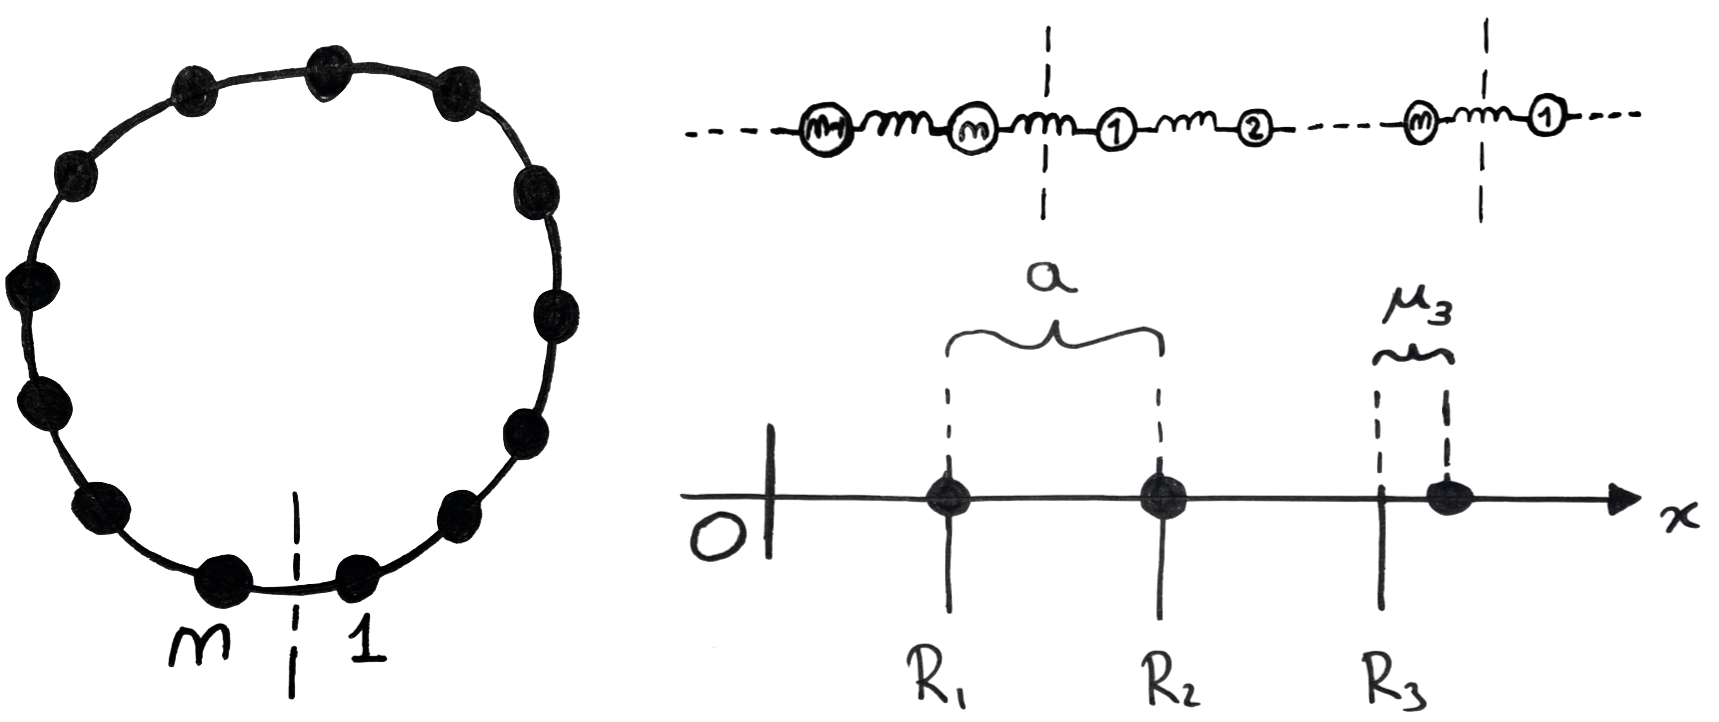
\includegraphics[scale=0.2]{/catena_unidim_atomi}
\caption{Catena unidimensionale di atomi}
\end{figure}

Poiché la catena è chiusa, si possono imporre condizioni al contorno periodiche.
Si ha che la forza di interazione tra due particelle è nulla, quando la molla è all'equilibrio e cioè quando $x_2-x_1 = a$.
\begin{equation}
F_{21} = - K (x_2 - x_1 - a) = - K (x_2 - R_2 - x_1 + R_1 + R_2 - R_1 - a) = - K (\mu_2 - \mu_1)
\end{equation}
Impostando le equazioni differenziali del moto, si ha che:
\begin{equation}
\begin{cases}
	m \ddot{x_2} = - K (\mu_2 - \mu_1) + K (\mu_3 - \mu_2) \\
	\ddot{x_2} = \ddot{\mu_2}
\end{cases}
\end{equation}
Dove la somma è dovuta è dovuta al fatto che quando la quantità al secondo membro è positiva,
l'interazione spinge la particella verso destra sull'asse $x$.
È dunque possibile scrivere l'equazione del moto generica per l'$n$-esima particella,
sulla quale però si approssima valutando solo le interazioni fra le particelle adiacenti.
\begin{equation}
\begin{split}
& m \ddot{\mu_n} = - K (\mu_n - \mu_{n-1}) + K (\mu_{n+1} - \mu_n) \Rightarrow \mu_n = S e^{ i K R_n } e^{ - i \omega t } \\
& \begin{cases}
	k = \frac{ 2\pi}{\lambda } \\
	\omega = 2\pi \nu \\
	R_n = n a
\end{cases} \\
& - \omega^2 m S e^{ i K_n a } e^{ - i \omega t } = - K S \Bigl(  e^{ i K_n a } - e^{ i K_{n-1} a } \Bigr) e^{ - i \omega t } + K S \Bigl(  e^{ i K_{n+1} a } - e^{ i K_n a }  \Bigr) e^{ - i \omega t }  \\
& \mbox{Dividendo a destra e sinistra per} \quad Q = - S e^{ i K_n a } e^{ - i \omega t } \\
& \omega^2 m = K \Bigl(  1 - e^{ -i K a }  \Bigr) + K \Bigl(  1 - e^{ i K a }  \Bigr) = K \Bigl[ 2 - 2 \cos(K a) \Bigr] \\
& \mbox{sfruttando ora la proprietà trigonometrica:} \quad \sin^2\Bigl(  \frac{ X}{2 }  \Bigr) = \frac{ 1}{2 } ( 1 - \cos(X) ) \quad \mbox{e si ottiene: } \\
& \omega^2 = \frac{ 4K}{m } \sin^2\Bigl(  \frac{ K a}{2 }  \Bigr) \Rightarrow \omega(K) = 2 \sqrt{\frac{ K}{m }} \Bigl|\sin \Bigl(  \frac{ K a}{2 }  \Bigr)\Bigr| \\
& \mbox{dove il valore assoluto si ha perché deve essere } \omega > 0
\end{split}
\end{equation}

Se si traccia il grafico della funzione trovata si ottiene:

% IMMAGINE

Se $\frac{ K a}{2 }$ è piccolo, cioè $\lambda$ è grande, si può sfruttare lo sviluppo in serie di Taylor e vedere che:
$ \omega (\frac{ Ka}{2 } \sim 0) \sim \sqrt{\frac{ K}{m }} |K a| = G K$
Questo significa che per $\frac{ Ka}{2 } \sim 0$ l'andamento della funzione è lineare, che è esattamente ciò che ci si aspetta nei mezzi continui, per cui la velocità di fase è uguale a quella di gruppo $\frac{ \omega}{K } = \frac{ d\omega}{dK } = \sqrt{\frac{ K}{m }}a$.
In tali condizioni infatti non si ha dispersione e per questo $\omega(K)$ è detta \underline{curva di dispersione}.
Un mezzo rimane non dispersivo finché $\lambda$ rimane grande, perché non si percepisce che il mezzo è discreto e non continuo.
Quando $K \sim \frac{ \pi}{ a}$ l'onda diventa stazionaria, poiché si annulla la velocità di gruppo.
Quando la curva abbandona l'andamento lineare, si ha il fenomeno della dispersione, come conseguenza della natura discreta del mezzo (la catena è formata da $N$ atomi).
Debye strutturò il suo modello, sostituendo la curva di dispersione con una linea dritta, assumendo che il mezzo fosse continuo, e introdusse la frequenza di taglio,
per tener conto della quantizzazione.

Sfruttiamo ora le condizioni al contorno periodiche:
\begin{equation}
\mu_{N+1} = \mu_1 \Rightarrow \mu = S e^{ i K a - i \omega t } = \mu_{N+1} = S e^{ i K a + i K N a - i \omega t } \Rightarrow e^{ i K N a } = 1 \Rightarrow K = \frac{ 2 \pi}{N a } l
\end{equation}
con $l \in \mathbb{Z}$, è possibile dire che ci sono solo $N$ valori di $K$ che portano ad $N$ soluzioni diverse, e ciò si vede se si fa variare di $\frac{ 2\pi}{a }$, perché si ottiene lo stesso risultato. 





















